\chapter{Introduction} 
This introduction contains the project goals and some very short introductions on the FPGAs and how they are used, numerical methods for approximating ODEs, functional programming and \clash{}. The goal of this report is to be understandable for any technical BSc student which is not necessarily familiar with functional programming, or numerical mathematics and therefore the short introductions are included for the sake of completeness and are assumed knowledge for the rest of the thesis. 

\section{Project goals}
From the start, this project has had two main goals: firstly, obtaining information on the feasibility and the advantages and disadvantages of performing numerical mathematics (specifically, solving ODEs \footnote{In this thesis, the term 'solving' will be used for both the process of solving an ODE analytically and for computing a numerical approximation to an ODE.}) directly on (programmable) hardware, the FPGA. Secondly: figuring out whether higher-order functions are of much use for numerical mathematics. As per usual, having main goals spawns off several minor goals which support the main parts. Both supporting goals are about simplifying the process of configuring FPGAs: an easy way of setting up projects with complicated IO requirements and furthermore, developing a toolchain integration which turns the long process of compiling and deploying your FPGA project into the execution of a single command.

Alongside these concrete goals the underlying theme is to do as much work as possible in \clash{}, a library and compiler based on the functional programming language Haskell, developed by Christiaan Baaij at the CAES group at the University of Twente. Further elaboration on \clash{} can be found in section \ref{s:clash}.


\section{FPGAs}
\subsection{What is an FPGA?}
An FPGA (Field Programmable Gate Array) is a chip in which you can specify the hardware yourself. In contrast to regular programming in which you generate a long list of instructions which are executed sequentially on a fixed chip configuration, the FPGA allows you to specify exactly which wire (signal) leads where and what operation should be applied to that signal. This approach to programming can have several advantages. The first one arises from the large opportunities for parallelism. Every part of the FPGA can be executing a meaningful computation simultaneously, whereas processors are bound by the amount of physical cores they have in the amount of truly concurrent instruction executions possible. Secondly, a conventional processor only has a fixed instruction set. Using an FPGA you can define your own instructions (subcircuits), again providing a possible improvement in computational speed. According to \cite{FPGAvsCPU}, FPGAs were already capable of outperforming CPUs on very parallelizable numerical tasks on single and double precision floating point numbers in as early as 2004. Furthermore, as you are implementing your signal processing directly in hardware, there will be a fixed bound on the possible latency. This makes FPGAs ideal for purposes in high-throughput, low-latency signal processing, eg. real-time audio, video or data stream processing. Lastly, the reconfigurability of FPGAs whilst remaining close to the actual hardware allows for cost reductions in the verification of ASIC (Application-Specific Integrated Circuits) designs. It's cheaper to reprogram your FPGA than to have a new version of an ASIC manufactured.

However, the FPGA is a trade-off between implementing designs directly in hardware and being able to run multiple designs (after a reconfiguration). As a consequence of this, it still loses to ASICs with several orders of magnitude on performance \cite{FPGAvsASIC} and CPUs still dominate in terms of versatility and on-the-fly reconfigurability.

\subsection{How does it work?}
An FPGA is built up from several distinct element types, depicted in figure \ref{f:fpga_fabric}
\begin{enumeratens}
	\item \emph{Logic elements} Responsible for the actual signal processing. An FPGA may contain different types of logic elements, eg. memory, DSP and logic blocks. These blocks implement some signal processing capability which can be configured up to certain limits.
	\item \emph{Programmable interconnects} In order to be able to represent complex designs, the logic elements need to be connected in a certain way. This is what the programmable interconnects are for. Essentially, those are wires which can be turned on and off by the user as part of a design specification. 
	\item \emph{IO blocks} Finally, the functionality implemented using the logic elements and programmable interconnects should be exposed to external signals in order to be useful. IO blocks can be used to control hardware pins, controlling a LED or reading a switch but also for more intricate IO facilities, eg. external memory controllers.
\end{enumeratens}

\begin{figure}[h]
	\centering
	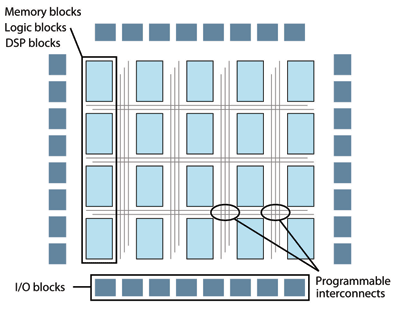
\includegraphics[width=0.5\textwidth]{fpga_fabric}
	\caption{FPGA fabric.}
	\label{f:fpga_fabric}
\end{figure}

It might seem that programming an FPGA involves manually specifying the interconnects and exact configurations of the logic elements. However, specialized languages have been developed just for the purpose of describing the FPGA functionality at a higher level of abstraction and leave the specific routing and assignment of logic elements to the compiler. The two main advantages of these languages are that you do not have to worry about low-level problems like how the interconnects will be routed and secondly, your written specification will be portable across multiple FPGA vendors as long as the vendor supplies you with the proper compiler from your specification to a file which can be used to program the FPGA. 

More information on FPGA functionality can be found in \cite{FPGAexplained}.


\subsection{System-on-a-chip}
FPGAs in itself can be useful, but especially for design with IO requirements that are more complex than just reading out hardware switches and controlling LEDs, more control is needed. This requirement has led to the rise of SoCs (System-on-Chip). These devices integrate an FPGA with additional hardware on a single chip. This extra hardware usually contains a CPU, which can be used to simplify the process of loading and extracting data from the FPGA. The SoC used for this thesis is the Terasic SoCKit, a development kit containing an Altera Cyclone V FPGA and a dual-core ARM A9 CPU on a single chip (Altera 5CSXFC6D6F31C6N), alongside a wide variety of IO possibilities. Further information on the SoC used is available at \cite{SoCKit}.

\section{Numerical solvers for ODEs}
The field of numerical solvers is a vast and active area of research. Furthermore, there is a lot of theory on which solver to pick for specific problems, related to stability, computational efficiency and other factors. However, the goal of this thesis is to get an impression of the feasibility of using numerical solvers for ODEs on FPGAs. Therefore, the selection of solvers will be restricted to some very basic schemes. 

The solvers used have some common properties:
\begin{itemizens}
	\item \emph{Fixed-step} - The solvers compute a value for the ODE at a fixed step size. This means that in contrary to the continous 'mathematical' solution of an ODE, the output of the solver will be an approximate to the actual value of the solution at the discrete set of values of the independent variable, in which the difference between the values of the independent variables is defined by the fixed step size.
	\item \emph{Single-step} - The approximate value of the ODE $x_{k}$ at $t_{k}$ only depends on $t_{k-1}$, $x_{k-1}$ and the ODE that is being approximated.   
\end{itemizens}

Both solvers work equally for both vectors and scalars. In case of a vector, the operations listed in \ref{eq:euler} and \ref{eq:rk2} should simply be applied to all elements of $\vec{x}$.

\subsubsection{Euler}
The easiest numerical solver, without doubt, is Euler's method (equation \ref{eq:euler}). For every discrete point in time, the value of the next point is approximately equal to the derivative at that point multiplied by the time step added to the current value. The simplicity of the scheme has a cost: it is not very accurate and the errors accumulate quickly. From \cite{DE}, the maximum error of Euler's method can be shown to be linear in the time step and exponential in the interval length (eq \ref{eq:euler_error}), in which $M$ and $L$ are constants depending on the equation to be solved, $b-a$ is the solution interval length and $h$ is the time step.

\begin{align}
	\label{eq:euler}
	s_{k,1} &= f(t_{k},x_{k}) \\
	x_{k+1} &= x_{k} + h s_{k,1} \nonumber
\end{align}

\begin{equation}
\label{eq:euler_error}
\text{maximum error}_{\text{euler}} \leq \frac{M h}{L} (e^{L(b-a)} -1)
\end{equation}

\subsubsection{Runge-Kutta}
The Runge-Kutta methods are a family of solvers, of which the 4th order version is the most well-known (RK4). The solver used here will be a second-order Runge-Kutta method, also known as the \emph{improved Euler's method} \cite{DE}. This second order method requires the computation of two slopes (equation \ref{eq:rk2}), in contrast to the single one required for Euler's method.

\begin{align}
	\label{eq:rk2}
	s_{k,1} &= f(t_{k},x_{k}) \\
	s_{k,2} &= f(t_{k} + h,x_{k} + h s_{k,1}) \nonumber \\
	x_{k+1} &= x_{k} + h \frac{s_{k,1} + s_{k,2}}{2} \nonumber
\end{align}

\begin{equation}
\label{eq:rk2_error}
\text{maximum error}_{\text{RK2}} \leq \frac{M h^{2}}{L} (e^{L(b-a)} -1)
\end{equation}

Note that the maximum error of RK2 is proportional to the square of the time step (equation \ref{eq:rk2_error}). As the time step decreases by a factor of 2, the maximum error will decrease by a factor of 4, given that the equation and the range stay the same. However, the maximum error still depends exponentially on the interval length.


\section{Functional programming}
\lstset{style=haskellStyle}
\subsection{What is functional programming?}
As the name suggests, the functional programming paradigm uses functions. These functions are used to build up the program and create structure. In contrast to the imperative programming paradigm, there is no assignment - there are only expressions. It is by evaluation of these expressions that you execute your program. These expressions consist of variables, constants and operations. However, the name variable may be ill-chosen, as assignment does not exist and therefore it is impossible for a variable to vary. Once you have bound a value to a certain variable, this value may not change and the value should be the same at every point where this variable is referenced (a concept called referential transparency). 

The exclusion of assignment from functional languages has several consequences. It becomes impossible to program using loops. The alternative is the use of recursive (listing \ref{lst:rec_function}) and higher-order functions (functions that have other functions as parameters or output). Especially higher-order functions have the side effect that they add clarity about the way the program functions (listing \ref{lst:ho_functions}). For instance, a \code{map} applies the same function to every element in a list, resulting in a new list. A \code{fold} would start at an initial value and element-by-element combine the list into a single value using a specified function, eg. addition. Both these operations would be implemented using a for-loop in an imperative language, but their goal is completely different. The availability of higher-order functions allows for more clarity in code by being able to specify exactly what kind of operation you want to perform. Another effect of the lack of assignment is the lack of side effects in functional programming. As there is no way to modify a variable, there is also no way of accidentally modifying a variable such that you enter an invalid state and other parts of the program stop functioning correctly.

\begin{lstlisting}[caption=Recursive functions, label=lst:rec_function]
fac :: Num a => a -> a
fac 0 = 1
fac n = n * fac(n-1)
\end{lstlisting}

\begin{lstlisting}[caption=Higher order functions, label=lst:ho_functions]
timesTwo :: Num a => [a] -> [a]
timesTwo xs = map (*2) xs

sum :: Num a => [a] -> a
sum xs = foldl (+) 0 xs

powers :: Num a => a -> a -> [a]
powers init power = iterate (\x -> x * power) init

powers100 = take 100 $ powers 1 2
\end{lstlisting}

The concept of higher-order functions also serves as an introduction to another very important concept in Haskell: the type system. Everything has a fixed type and often times, when only looking at the type definition you can already guess what the function is going to do. Consider the type signature of \code{map} in listing \ref{lst:haskell_types}. It requires a \code{(a->b)}, a function to turn something of type \code{a} into something of type \code{b}. Furthermore, it needs a list of \code{a}, \code{[a]} (indicated by the square brackets) and it returns something of type 'list of b' (\code{[b]}). The type signature of the \code{foldl} is slightly harder to understand, but it requires a function which needs an \code{a} and a \code{b} to produce a new \code{b}. Furthermore, an initial value (\code{a}) and a list of b to operate on (\code{[b]}) in order to return the final result, which has again type \code{a}. Function type signatures can be daunting to understand at first, but not all of them are as complicated as the \code{foldl}. For instance, a function which can be used to represent a differential equation, which needs a state of the system (the \code{ODEState}) in order to compute the derivative at that point (the \code{D_ODEState}). As a last example, the type signature of \code{Solver}: it requires some integration scheme, settings for the time (initial time and a time step), it requires an equation and an initial state of the system. All of this combined results in a list of states: the numerical approximation to the solution of the ODE. Note that in this example, the integration scheme \code{Scheme} itself is a function, for which understanding the type signature should pose no problem by now.

The last concept in functional programming which is important to understand is so-called lazy evaluation. In contrast to imperative programming, a value is only evaluated whenever it is needed. For instance, this allows for the concept of an infinite list, which is definitely not attainable in imperative programming as it would run out of memory. An example of this is the higher-order function \code{iterate}, shown in listing \ref{lst:ho_functions}, as part of the \code{powers} function. This function generates an infinite list by repeatedly applying a function (in this case a multiplication by a constant) to its own output, starting at the initial value \code{init}. However, it would be impossible to actually display the entirety of said infinite list and therefore you apply another function, \code{take n}, which only consumes the first \code{n} elements of a list. As the total evaluation only requires the first \code{n} elements, these are the only ones that will actually be computed. \cite{FPintro}

\begin{lstlisting}[caption=Type signatures, label=lst:haskell_types]
map :: (a->b) -> [a] -> [b]
foldl :: (a->b->a) -> a -> [b] -> a

type Equation = ODEState -> D_ODEState
type Scheme   = TimeSettings -> Equation -> ODEState -> ODEState
type Solver   = Scheme -> TimeSettings -> Equation -> ODEState  -> [ODEState]
\end{lstlisting}

\subsection{Using FP for numerical mathematics}
Functional languages have several properties which make them suitable for the purpose of solving problems in numerical mathematics. First and foremost, Haskell, being based on $\lambda$-calculus is very close to mathematics. The useful mathematical properties here are \textit{referential transparency}, easy \textit{partial function application} and being a \textit{declarative language}. 
Referential transparency implies that a variable only has a constant value which is the same everywhere in the program. This prevents that changing a variable might have influence on another computation as a side effect and it corresponds to mathematical notation. For instance, in an imperative programming like C you could write \code{i = i + 1}, which is a mathematical impossibility and therefore not allowed in Haskell. 
Partial function application is another very useful concept. Often in numerical mathematics, you want to create or process a function. You need a function that has another function as return value. For instance, take a function which requires two arguments. After only applying a single argument, the object returned still needs the second argument in order to compute the final value. This is exactly according to the definition of a function: An object that still needs arguments before being able to return its final value.
Being a \textit{declarative language} means that you write code that specifies what you want to accomplish, not how to get there. This concept is again borrowed from mathematics. You put in a set of function definitions and Haskell will figure out how to actually compute the value you request according to those definitions. This property of declarativity also has the result that Haskell is a terse language whilst remaining easy to understand.
Secondly, Haskell has a very strong type system. The type system has three main advantages. It becomes very easy to swap out and replace functions as long as you make sure that the types are the same. The Haskell compiler will start to assert errors immediately whenever you feed it something which does not make sense or could be ambiguous which is very useful when writing programs. By having a look at the types of a Haskell program it becomes very straightforward to see what the program does and how it works, which is very useful when attempting to understand your own or someone else's code.
Lastly, a property which is often very important for numerical mathematics: Haskell is fast. According to the \textit{Computer Language Benchmarks Game} \cite{Bench}, Haskell is almost on par with Java and Fortran but significantly faster than Python and Matlab (not shown), two languages which are often used for numerical mathematics nowadays. There is still a performance gap of around a factor 3 between Haskell and C (the reference), hence if speed is of the absolute highest concern C is still a valid option.

\subsection{Example: Numerical solutions of ODEs in Haskell}
\label{s:numsolHaskell}
As mentioned before, the types in Haskell reveal lots of information about the structure and functionality of the program. The three main types constituting the numerical solver for ordinary differential equations are listed in listing \ref{lst:solvertypes}.

\lstinputlisting[caption=Main types for the ODE solver, label=lst:solvertypes, firstline=18]{../haskell/SolverTypes.hs}

\subsubsection{Equation}
In essence, a differential equation is a mapping (function) from a certain state of the system to the change of this system. This is also what the type signature of \code{Equation} signifies, a mapping from an \code{ODEState} to a \code{D_ODEState}, the change in state or the derivative. This generic set up allows the specification of any ODE for solving. The implementation in pure Haskell of a simple ODE is given in listing \ref{lst:eq_exponential}, which corresponds to the equation $x' = -x$. However, this representation is not very elegant and a lot of the code is performing unboxing of the types. Using property that this equation is linear, it is possible to use an utility method which takes as input a matrix and returns the Haskell differential equation function belonging to that matrix. The same can be done for heterogeneous linear systems using a different utility function, which does not only takes a matrix as input but also a list of functions representing the heterogeneous part of the equation.

\lstinputlisting[caption=Example equation for exponential decay, label=lst:eq_exponential, firstline=11,lastline=14]{../haskell/SolverEquations.hs}

\subsubsection{SolveMethod}
The \code{SolveMethod} performs the actual computations on what the next value of the solution should be: the integration scheme. In order to obtain this next state, the scheme needs three input values: It needs information on the timing constraints of the solution, in this case it needs the time step. Furthermore, it needs the equation itself and it requires the state of the system at $t_{n}$ in order to be able to determine the state of the system at $t_{n+1} = t_{n} + \Delta t$.

The most straightforward integration scheme is called forward Euler, given in equation \ref{eq:euler}. Listing \ref{lst:euler} depicts the translation of the mathematical expression \ref{eq:euler} to Haskell. Even though some list operations have been inserted (\code{zipWith} and \code{map}), the structure is still recognizable. It computes the change in state, multiplies this with the time step obtained in line 6 and adds the initial state in line 4. Lastly, the integration scheme returns the new state of the equation, consisting of a list of x-values and a corresponding time value. Implementations of different solvers (i.e. 4th order Runge-Kutta) can be found in appendix \ref{app:haskellsolver}.

\lstinputlisting[caption=Example code for the Euler integration scheme, label=lst:euler, firstline=9,lastline=15]{../haskell/SolverSolvers.hs}

\subsubsection{Solver}
The \code{Solver} function in listing \ref{lst:solver_frame} acts as the main interface to the program. You specify a \code{SolveMethod}, the \code{TimeSettings} (containing the time step and the time at which to stop solving), the equation itself and an initial condition. The \code{Solver} will then return a list of states of the system. This problem could be solved recursively, but a method featuring more clarity is a higher-order function, in this case \code{iterate}. This function keeps applying itself to its own output, starting with some specified initial value, generating an infinite list. However, we are not interested in the infinite list of solutions and therefore we only take the first N elements, in which N depends on the initial time, the final time and the time step used for the solution.

The solutions of a wide range of equations, both linear and non-linear, both homogeneous and heterogeneous and using the input matrix utility functions have been plot with suitable initial conditions to show their behavior in figure \ref{f:solver_example}.

\lstinputlisting[caption=The main controlling function, label=lst:solver_frame, firstline=14,lastline=18]{../haskell/Solver.hs}

\subsubsection{Results}
This example of approximating solutions to ODEs using Haskell shows the versatility the language and especially its type system. Without any trouble, it is possible to exchange solver schemes, equations, settings and initial conditions by merely changing a single identifier in the function call. A variety of equations with suitable initial conditions have been approximated: both linear and non-linear, of multiple orders, both homogeneous and heterogeneous. As an example, the equations of which the solutions (with suitable initial conditions) are depicted in figure \ref{f:solver_example} are listed in equations \ref{eq:overview}. The exact Haskell source generating the plot is shown in \ref{app:haskellsolver}, but depends on an external library for generating the plot \cite{HaskellChart}.

\begin{align}
	\label{eq:overview}	
	\text{Exponential}\sep{}			x(t)' &= -x(t)  \nonumber \\
	\text{Simple harmonic}\sep{}		x(t)'' &= -x(t) \nonumber \\
	\text{Cosine hyperbolic}\sep{}		x(t)' &= \frac{\sqrt{x(t)^{2} - a^{2}}}{a} \\
	\text{Simple harmonic}\sep{}		\vecb{x}(t)' &= \begin{bmatrix} 0 & 1 \\ -1 & 0 \\ \end{bmatrix}\vecb{x}(t) \nonumber \\
	\text{Simple forced harmonic}\sep{}	\vecb{x}(t)' &= \begin{bmatrix} 0 & 1 \\ -1 & 0 \\ \end{bmatrix}\vecb{x}(t) + \begin{bmatrix} \sin{(t)} \\ e^{-t} \\ \end{bmatrix} \nonumber
\end{align}

\begin{figure}[h!]
	\centering
	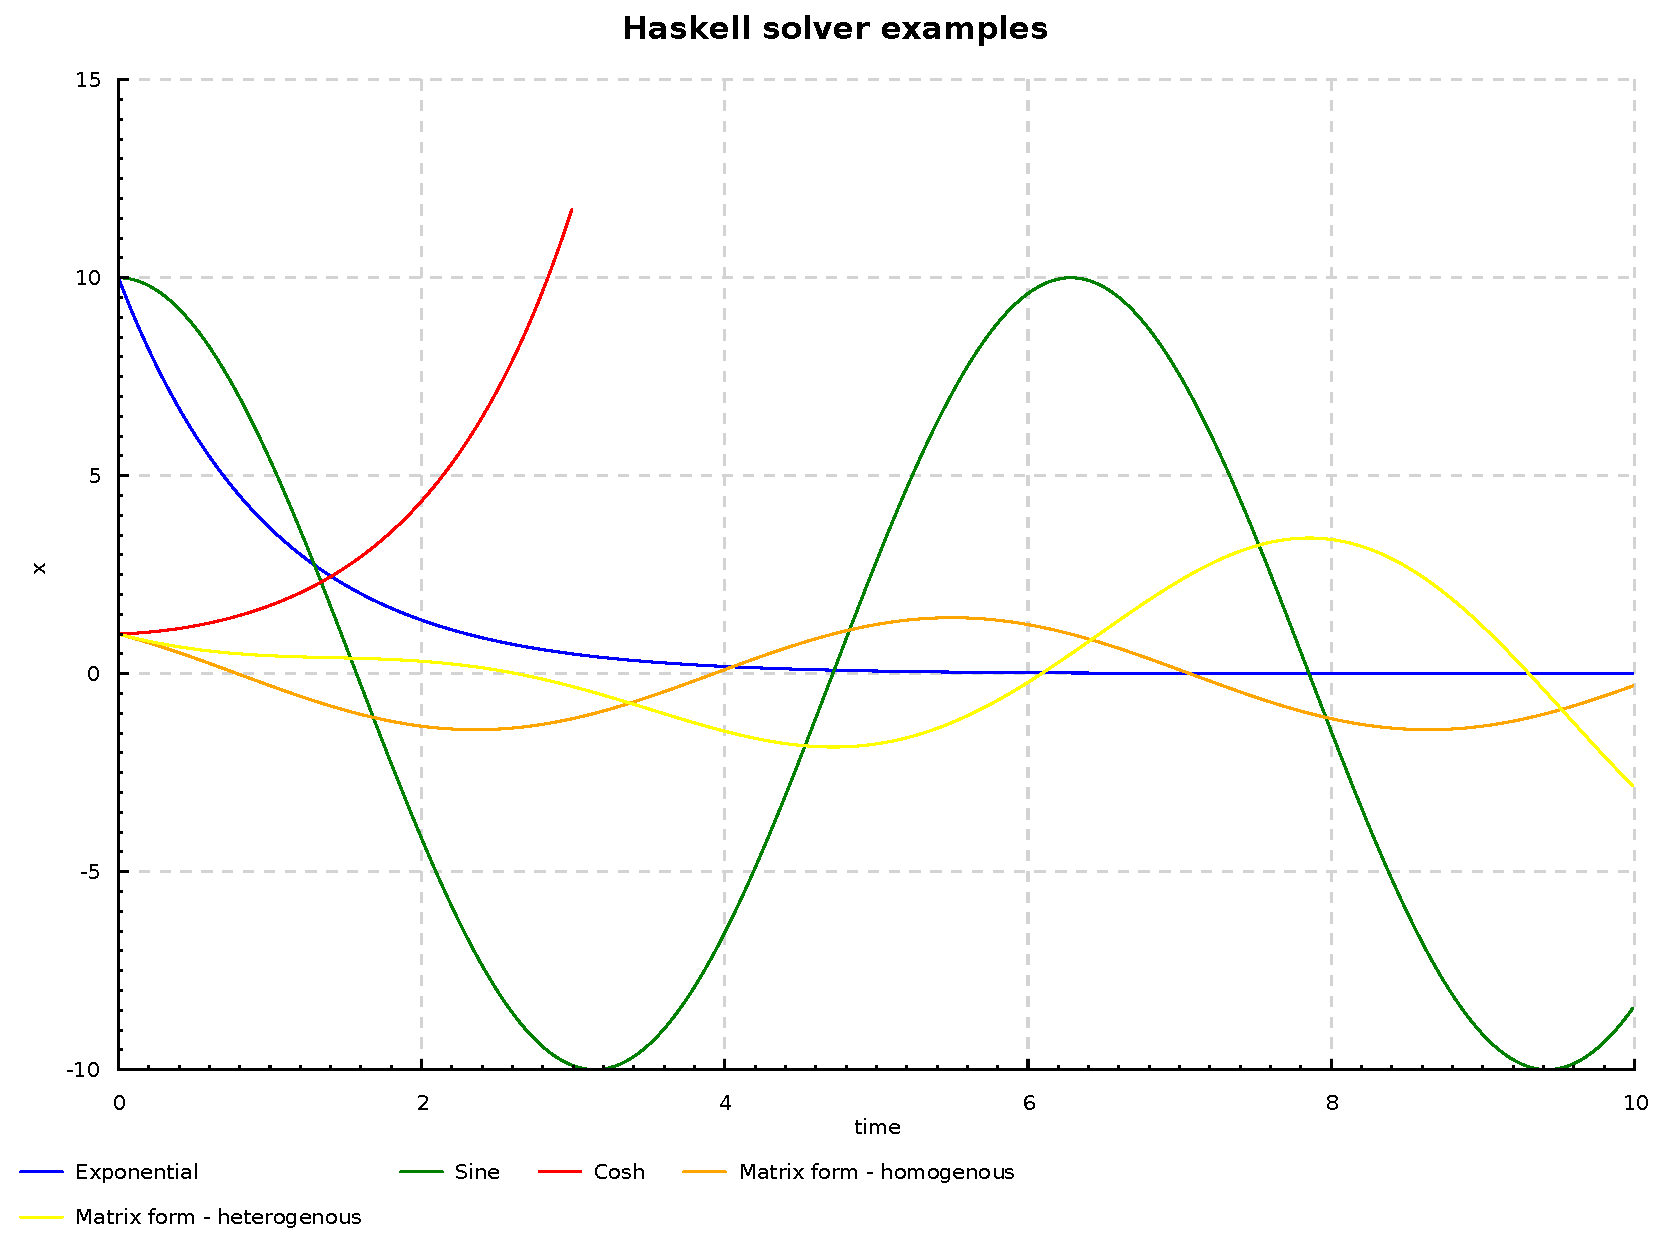
\includegraphics[width=\textwidth]{../haskell/haskell.pdf}
	\caption{Plots of the ODE solutions, simulated in Haskell.}
	\label{f:solver_example}
\end{figure}


\section{\clash{}}
\label{s:clash}
Functional programming has several aspects in common with hardware design, which was the original reason for the development of \clash{}, a library and special compiler which is capable of compiling a subset of Haskell into HDL. In \clash{}, every (sufficiently complex) hardware design consists of two parts: a combinatorial part and a synchronous part. It is the combinatorial part which can be modeled with few problems in a functional way: there is no time dependency - the output is merely an evaluation of a certain function of the inputs and for every input the output will be the same. However, complex hardware designs do not merely consist of stateless combinatorial circuits, in order to perform work some statefulness must be included. This is the task of the synchronous part of the design, keeping track of the state. The state is often implement using latches or memory cells which can get updated with new values, computed by the combinatorial part, every clock cycle (hence the name synchronous part). Together, the combinatorial part and the synchronous part of hardware are called sequential logic: the output depends on both the current input and the past inputs.

\begin{figure}[h]
	\centering
	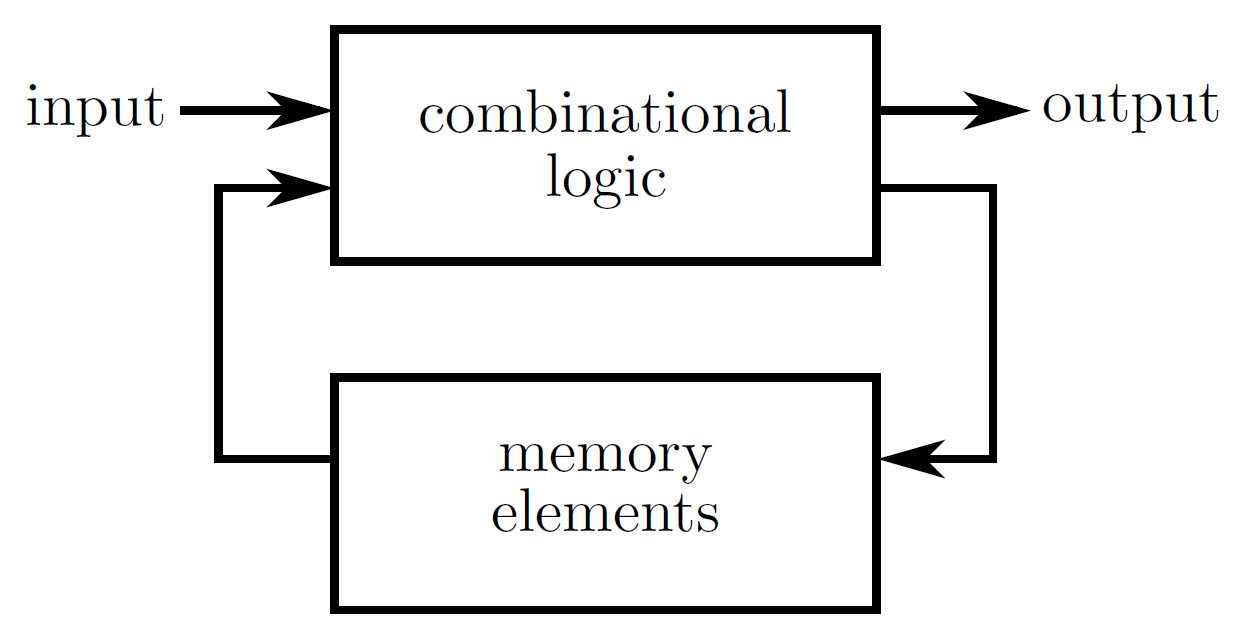
\includegraphics[width=0.5\textwidth]{mealy_machine}
	\caption{A flowchart of the Mealy machine}
	\label{f:mealy_machine}
\end{figure}

\subsection{Mealy machines}
It is the synchronous (statefulness) part that cannot be modeled directly in Haskell, but \clash{} gets around this by use of the Mealy machine \cite{BaaijMSc}. On every clock cycle, based on the input and the current state the combinational logic computes an output and a new state. The updated state gets stored in the memory elements, the output forwarded to the external ports of the hardware. When looking at some \clash{}-Haskell, this structure of generating an output and a new state based on an input and the current state is still clearly visible, for example in listing \ref{lst:clash_basic}. After defining a function with the proper type signature for a Mealy machine you can pass this function to the \clash{} built-in function \code{mealy}, which handles the conversion to a valid \code{topEntity}. In this case the specified function is multiply-accumulate, which, for every clock cycle, multiplies its inputs together and adds it to an internal sum which gets forwarded to the output. \cite{CLaSHTut}


\begin{lstlisting}[caption=A basic example a multiply-accumulate specification in CλaSH, label=lst:clash_basic]
topEntity :: Signal (Signed 9, Signed 9) -> Signal (Signed 9)
topEntity = mealy mac initial

mac state input = (state',output)
  where
    (x,y)   = input         -- unpack the two inputs
    state'  = state + x*y   -- the new state
    output  = state'        -- output the new state
\end{lstlisting}

\subsection{Advantages of \clash{}}
The power of \clash{} is manifold. Firstly, you are writing valid Haskell code, which allows you to simulate and verify your designs by relying on existing debugging techniques for Haskell. Secondly, Haskell enables more clarity in code, partially by use of higher-order functions, partially by use of it's record syntax, which allows you to easily group signals together in a meaningful way. This additional clarity is especially useful in complex designs in combination with the modularity of functional programs (as long as you adhere to the type signature), which allows you to easily swap out parts of design. Thirdly, notice that the only location at which the types of the signals has been specified is in the first line (\code{Signed 9}, a signed integer of length 9). This means that, in order to have our multiply-accumulate circuit work on, for instance, unsigned integers of length 32, the only place that needs modification is the \code{topEntity} function type signature. The other types are inferred from here.


After specifying your design in \clash{}, you can invoke the \clash{}-compiler to generate HDL. Both mainstream languages (VHDL and Verilog) are supported. It is then the HDL which can be compiled by a vendor-specific compiler into a binary file which can be flashed to the FPGA. 
